\documentclass[english,compress]{beamer}
\usepackage{kloeckislides}
\nonstopmode

\usepackage[normalem]{ulem}
%\useoutertheme{split}
%\useinnertheme{rectangles}
%\usecolortheme{owl}
%\usetheme{Singapore}

\usepackage{pifont}
\usepackage{ifthen}

\setbeamercolor{section in head/foot}{use=structure,bg=structure.fg!25!bg}
\defbeamertemplate*{footline}{split theme}
{%
  \leavevmode%
  \begin{beamercolorbox}[wd=.5\paperwidth,ht=2.5ex,dp=1.125ex]{section in head/foot}%
    \insertsectionnavigationhorizontal{\paperwidth}{\hskip0pt plus1filll}{}%
  \end{beamercolorbox}%
  %\begin{beamercolorbox}[wd=.5\paperwidth,ht=2.5ex,dp=1.125ex]{subsection in head/foot}%
    %\insertsubsectionnavigationhorizontal{.5\paperwidth}{}{\hskip0pt plus1filll}%
  %\end{beamercolorbox}%
}


%\useoutertheme[subsection=false]{miniframes}

\setbeamertemplate{frametitle}[default][center]

\AtBeginDocument{%
  {
    \usebeamercolor{section in head/foot}
  }
  
  \pgfdeclareverticalshading{beamer@headfade}{\paperwidth}
  {%
    color(0cm)=(bg);
    color(1.25cm)=(section in head/foot.bg)%
  }

  \setbeamercolor{section in head/foot}{bg=}
}

\addtoheadtemplate{\pgfuseshading{beamer@headfade}\vskip-1.25cm}{}

\beamertemplatedotitem

\setbeamercolor{section in head/foot}{parent=palette quaternary}
\setbeamercolor{subsection in head/foot}{parent=palette primary}

\setbeamercolor{author in head/foot}{parent=section in head/foot}
\setbeamercolor{title in head/foot}{parent=subsection in head/foot}



\AtBeginSection[] {
  \begin{frame}<beamer>
  \frametitle{Outline}
  \tableofcontents[sectionstyle=show/shaded,subsectionstyle=show/show/hide]
\end{frame}
}
\AtBeginSubsection[] {
  \begin{frame}<beamer>
  \frametitle{Outline}
  \tableofcontents[sectionstyle=show/shaded,subsectionstyle=show/shaded/hide]
\end{frame}
}

\newcommand{\technicality}[2]{%
  {\strut #1\\
    \begin{beamercolorbox}[sep=1mm]{block body}
      #2
    \end{beamercolorbox}
  }%
}

\lstset{
  language=C++,
  rangebeginprefix=//\ ,
  rangeendprefix=//\ ,
}

\def\weblink#1#2{\href{#1}{\color{blue}\underline{#2}}}

\definecolor{fetch}{RGB}{227,110,35}
\definecolor{alu}{RGB}{255,188,24}
\definecolor{context}{RGB}{132,146,175}

\usepackage{keystroke}

\setbeamertemplate{navigation symbols}{}

\def\hilite<#1>#2{\alt<#1>{\colorbox{blue!30}{#2}}{\colorbox{white}{#2}}%
}

\lstset{
  language=C++,
  rangebeginprefix=//\ ,
  rangeendprefix=//\ ,
}

\colorlet{input}{green!30}
\colorlet{output}{red!30}
\colorlet{intermed}{blue!30}

\tikzset{
  input/.style={circle,fill=input,draw,thick,minimum height=4.5ex},
  output/.style={circle,fill=output,draw,thick,minimum height=4.5ex},
  func/.style={->,thick},
}

\begin{document}
% {{{ front matter

\title{High-Performance Scientific Computing\\Lecture 12: GPU Performance, Applications}

\date{MATH-GA 2011 / CSCI-GA 2945 $\cdot$ November 28, 2012}

\frame{\titlepage}

\begin{frame}{Today}
  \tableofcontents[hideallsubsections]
\end{frame}
% }}}
% -----------------------------------------------------------------------------
\begin{comment}
\begin{frame}{Bits and pieces}
  \begin{itemize}
    \item Don't have a project? Let's fix that \emph{very soon}
    \item HW5: soon
    \item HW6: due today
    \item Dec 5: Last day of regular class
    \item Dec 12: Legislative Day
    \item Dec 17/18/\textbf{19}: Project presentations
    \item Don't have grade reports for HW1\dots4? Talk to me
  \end{itemize}
\end{frame}
\end{comment}

% -----------------------------------------------------------------------------
\section{GPU performance}
% -----------------------------------------------------------------------------
% {{{
% -----------------------------------------------------------------------------
\subsection{Understanding GPUs}
% -----------------------------------------------------------------------------
\begin{frame}{Recap}
  \begin{itemize}[<+->]
    \item SIMD performance impact?
    \item How can GPU code deal with latency?
    \item Difference: \# FPUs / \# scheduling slots?
  \end{itemize}
\end{frame}
% -----------------------------------------------------------------------------
\begin{frame}{Comparing architectures}
  \begin{tabular}{l|cccc|l}
    & Nvidia & Nvidia & Nvidia & AMD & Units\\
    & GF100 & GF104 & GK104 & GCN & Units\\
    \hline
    \# Warps/core & 48 & 48 & 64 & 40\\
    Warp Size & 32 & 32 & 32 & 64 & W.Item \\
    SP FPUs/core & 32 & 48 & 192 & 64 \\
    Cores & 15 & 7 & 8 & 32 \\
    \hline
    Core clock & 1400 & 1300 & 823 & 925 & MHz \\
    \hline
    Reg File & 128 & 128 & 256 & 256 & kiB \\
    Lmem/core & 64  & 64 & 64 & 64 & kiB \\
    Lmem BW/core & 64  & 64 & 128 & 128 & B/clock \\
    \hline
    GMem Bus & 384 & 256 & 256 & 384 & Bits\\
    GMem Clock & 3696 & 3600 & 6008 & 5500 & MHz\\
    \hline
  \end{tabular}
  \creditto{David Kanter / Realworldtech.com}
  \uncover<+->{}
  \uncover<+->{
    \begin{tikzpicture} [overlay]
      \node [above left=1cm of current page.south east,draw,drop shadow,fill=white,
       inner sep=5mm,thick,text width=0.6\textwidth]
        {
          What are the main limits for programs?

          \bigskip
          What happens if you exceed them?
        } ;
    \end{tikzpicture}
  }
\end{frame}
% -----------------------------------------------------------------------------
\begin{frame}{Architecture}
  \begin{center}
    \Huge Occupancy calculator
  \end{center}
\end{frame}
% -----------------------------------------------------------------------------
\begin{frame}{Performance in three sentences}
  \begin{center}
    \Large
    Flops are cheap\\
    Bandwidth is money\\
    Latency is physics
  \end{center}
  \hfill [M. Hoemmen]
\end{frame}
% -----------------------------------------------------------------------------
\subsection{GPUs and Memory}
% -----------------------------------------------------------------------------
\input{parallel-memories}
\input{cl-gmem-access}
% -----------------------------------------------------------------------------
\begin{frame}{GPU Global Memory}
  \begin{center}
  \Huge GPU global access patterns demo
  \end{center}
\end{frame}
% -----------------------------------------------------------------------------
\input{cl-lmem-access}
% -----------------------------------------------------------------------------
\begin{frame}{GPU local Memory}
  \begin{center}
  \Huge GPU local access patterns demo
  \end{center}
  \uncover<+->{}
  \uncover<+->{
    \begin{tikzpicture} [overlay]
      \node [above left=1cm of current page.south east,draw,drop shadow,fill=white,
       inner sep=5mm,thick,text width=0.6\textwidth]
        {
          What does this mean for 2D arrays in local memory? (E.g. matrix transpose?)

          \only<+->{
            \bigskip
            What does this mean for \texttt{double}s in local memory?
          }
        } ;
    \end{tikzpicture}
  }
\end{frame}
% -----------------------------------------------------------------------------
{
  \newcommand{\brick}[6]{
    \draw [fill=#4!50]
      (0,0) rectangle (#1,#2) coordinate [pos=0.5] (brickfront);
    \draw [fill=#4]
      (#1,0) -- (#1,0,-1) -- (#1,#2,-1) -- (#1,#2) --cycle;
    \draw [fill=#4]
      (0,#2) -- (0,#2,-1) -- (#1,#2,-1) -- (#1,#2) --cycle;
    #6
    \begin{pgfonlayer}{foreground}
      \node [fill=#4!50,inner xsep=2pt,inner ysep=2pt,opacity=0.7,#5] at (brickfront) { #3 } ;
      \node [#5] at (brickfront) { #3 } ;
    \end{pgfonlayer}
  }
  \newcommand{\drawevt}[2]{
    \fill [#2,opacity=0.5]
      (0,#1) -- (1.5,#1) -- (1.5,#1,-1)
      -- (1.5,#1+0.2,-1) -- (1.5,#1+0.2) -- (0,#1+0.2) --  cycle ;
  }
  \begin{frame}{Faster transfers Host $\leftrightarrow$ GPU}
    \begin{columns}
      \column{0.55\textwidth}
        How about host $\leftrightarrow$ device transfers?
        \begin{itemize}
          \item If talking to CPU: Unnecessary
            \uncover<2->{\texttt{CL\_MEM\_ALLOC\_HOST\_PTR}}
          \item If talking to GPU:

            \medskip
            \begin{itemize}
              \item Want asynchronous transfer
              \item Want overlapping transfer
            \end{itemize}

            \medskip
            What about paging?

            \uncover<3->{
              \texttt{CL\_MEM\_ALLOC\_HOST\_PTR}

              \medskip
              (`pinned' memory--Demo)
            }
        \end{itemize}

      \column{0.4\textwidth}
        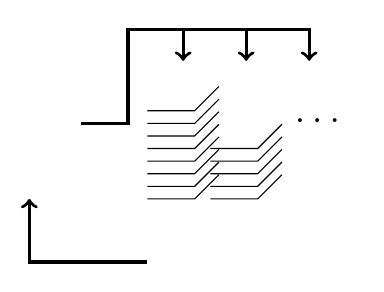
\begin{tikzpicture}[scale=0.8]
          \brick{1.25}{2}{Host}{gray}{}{}
          \begin{scope}[xshift=2.5cm,yshift=-1.5cm]
            \brick{2.5}{1.25}{Device}{gray}{}{}
          \end{scope}
          \begin{scope}[xshift=2.5cm]
            \brick{0.75}{2}{Queue 1}{blue}{text=white,rotate=90}{
              \foreach\i in {0,0.2,...,1.4}
                \draw (0,\i) -- (0.75,\i) -- (0.75,\i,-1);
            }
          \end{scope}
          \begin{scope}[xshift=3.5cm]
            \brick{0.75}{2}{Queue 2}{blue}{text=white,rotate=90}{
              \foreach\i in {0,0.2,...,0.9}
                \draw (0,\i) -- (0.75,\i) -- (0.75,\i,-1);
            }
          \end{scope}

          \node [font=\Large] at (5.25,1.25) {\dots} ;

          \draw [very thick,->] (1.25,1,-0.5) -| (2,2.5,-0.5) -| (2.875,2,-0.5);
          \draw [very thick,->] (2,2.5,-0.5) -| (3.875,2,-0.5);
          \draw [very thick,->] (2,2.5,-0.5) -| (4.875,2,-0.5);
          \draw [very thick,->] (2.5,-1) -| (0.625,0);
        \end{tikzpicture}
    \end{columns}
  \uncover<4->{
    \begin{tikzpicture} [overlay]
      \node [above left=1cm of current page.south east,draw,drop shadow,fill=white,
       inner sep=5mm,thick, text width=0.6\textwidth]
        {
          Important: Two different mechanisms at work!
        } ;
    \end{tikzpicture}
  }
  \end{frame}
}
% -----------------------------------------------------------------------------
\begin{frame}{Too little memory?}
  \begin{center}
    \Large
    Efficient code organization for out-of-core calculations?
  \end{center}

  \bigskip
  \textbf{Assume:} $\leftarrow$, $\rightarrow$ transfers, computation all
  proceed independently.

  \pause

  \begin{center}
    \Large
    ``Double buffering''
  \end{center}

  \emph{Idea:} Just keep everybody busy.

  \uncover<+->{}
  \uncover<+->{
    \begin{tikzpicture} [overlay]
      \node [above left=1cm of current page.south east,draw,drop shadow,fill=white,
       inner sep=5mm,thick,text width=0.6\textwidth]
        {
          Q: Describe that in OpenCL without synchronizing the host to
          the GPU.
        } ;
    \end{tikzpicture}
  }
\end{frame}
% -----------------------------------------------------------------------------
\begin{frame}{Entertainment: GPU Memory Zoo}

  \uncover<+->{
    \begin{tabular}{p{5em}cccp{2.8cm}}
    \hline
    \textbf{Type} & \textbf{Per} & \textbf{Access} & \textbf{Latency} \\
    \hline
    \textbf<2->{private} & work item & R/W & 1 or 1000 \\
    \textbf<2->{local} & group & R/W & 2 \\
    \textbf<2->{global} & grid & R/W & 1000 & Cached?\\
    \texttt{constant} & grid & R/O & 1-1000 & Cached \\
    image$n$d\_t & grid & R(/W) & 1000 & Spatially cached\\
    \hline
    \end{tabular}
  }
\end{frame}
% -----------------------------------------------------------------------------
\subsection{Summary}
% -----------------------------------------------------------------------------
\begin{frame}{GPU performance summary}
  \begin{itemize}
    \item Latency, latency, latency!
      \begin{itemize}
        \item Various forms: Memory, branches, computation
        \item All need to be hidden
      \end{itemize}
    \item Bandwidth: usually fixable
    \item Watch your memory access patterns
      \begin{itemize}
        \item Local mem is somewhat more forgiving
        \item \dots and lower latency, higher BW
      \end{itemize}
  \end{itemize}
\end{frame}
\begin{frame}{Demo}
  \begin{center}
  \Huge GPU profiler demo
  \end{center}
\end{frame}

% }}}
% -----------------------------------------------------------------------------
\section{MPI performance}
% -----------------------------------------------------------------------------
% {{{
\begin{frame}{MPI}
  \begin{center}
  \Huge MPI performance demo
  \end{center}
\end{frame}
% }}}
% -----------------------------------------------------------------------------
\long\def\sectionslide#1#2#3#4{
  \begin{frame}
    \begin{center}
      {\Huge \textless #1
      {\fontsize{130}{150}\fontfamily{phv}\selectfont #2}
      \textgreater}

      \vspace{1.5cm}
      \textbf{#3}

      \medskip\footnotesize
      #4
    \end{center}
  \end{frame}
}
\sectionslide{/}{2}{Understanding Computational Cost}{}
\sectionslide{}{3}{Concepts, Patterns and Recipes}{}
% -----------------------------------------------------------------------------
\section{Parallel Patterns}
% -----------------------------------------------------------------------------
\begin{frame}{Patterns: Overview}
  Parallel Programming:
  \begin{itemize}
    \item To what problems does it apply?
    \item How?
      \subitem{How big of a headache?}
    \item What mechanism is suitable?
  \end{itemize}

  \bigskip
  Organize discussion by patterns of \textbf{Dependencies}.
  \uncover<+->{}
  \uncover<+->{
    \begin{tikzpicture} [overlay]
      \node [above left=1cm of current page.south east,draw,drop shadow,fill=white,
       inner sep=5mm,thick]
        {
          Will move to more of a \emph{discussion} style
        } ;
    \end{tikzpicture}
  }
\end{frame}
% -----------------------------------------------------------------------------
\subsection[Embarrassing]{Embarrassingly Parallel}
% -----------------------------------------------------------------------------
% {{{
\begin{frame}{Embarrassingly Parallel}
  \uncover<+>{}
  {\Huge
  \[
    y_i = f_i(x_i)
  \]}%
  where $i\in\{1,\dots,N\}$.

  \medskip
  Notation: (also for rest of this lecture)
  \begin{itemize}
    \item $x_i$: inputs
    \item $y_i$: outputs
    \item $f_i$: (pure) functions (i.e. \emph{no side effects})
  \end{itemize}

  \medskip
  \uncover<+>{
    \begin{tikzpicture} [overlay]
      \node [below left=1cm of current page.north east, draw,drop shadow,fill=white,
      text width=0.75\textwidth, inner xsep=0.5cm,inner ysep=0.5cm,thick]
        {
          When does a function have a ``side effect''?

          \bigskip
          In addition to producing a value, it
          \begin{itemize}
          \item modifies non-local state, or
          \item has an observable interaction with the outside world.
          \end{itemize}
        } ;
    \end{tikzpicture}
  }%
  \uncover<+(1)->{
  Often: $f_1=\dots=f_N$. Then
  \begin{itemize}
    \item Lisp/Python function \texttt{map}
    \item C++ STL \texttt{std::transform}
  \end{itemize}
  }
\end{frame}
% -----------------------------------------------------------------------------
\begin{frame}{Embarrassingly Parallel: Graph Representation}
  \begin{center}
    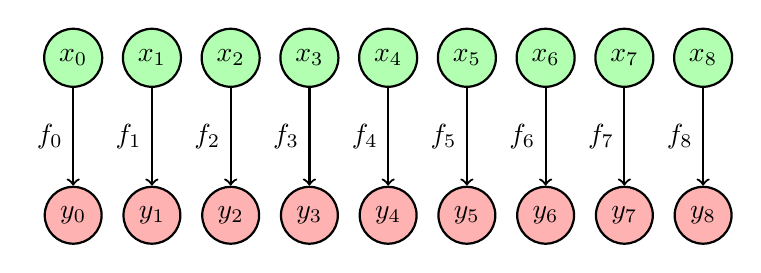
\begin{tikzpicture}
      \foreach \i in {0,1,...,8}
      {
        \node [input] at (\i, 0) (x\i) { $x_{\i}$ };
        \node [output] at (\i, -2) (y\i) { $y_{\i}$ };
        \draw [func] (x\i) -- (y\i) node [pos=0.5,anchor=east] {$f_{\i}$};
      }
    \end{tikzpicture}
  \end{center}
  \uncover<2>{
    \begin{tikzpicture} [overlay]
      \node [above left=1cm of current page.south east, draw,drop shadow,fill=white,
      text width=0.4\textwidth, inner xsep=0.5cm,inner ysep=0.5cm,thick]
        {
          Trivial? Often: no.
        } ;
    \end{tikzpicture}
  }
\end{frame}
% -----------------------------------------------------------------------------
\begin{frame}{Embarrassingly Parallel: Examples}
  \begin{columns}
    \column{0.6\textwidth}
      Surprisingly useful:
      \begin{itemize}
        \item Element-wise linear algebra:

          Addition, scalar
          multiplication (\emph{not} inner product)
        \item Image Processing: Shift, rotate, clip, scale, \dots
        \item Monte Carlo simulation
        \item (Brute-force) Optimization
        \item Random Number Generation
        \item Encryption, Compression

          (after blocking)
      \end{itemize}
    \column{0.4\textwidth}
      \includegraphics[width=\textwidth]{parallel-field.jpeg}
  \end{columns}
  \uncover<2>{
    \begin{tikzpicture} [overlay]
      \node [above left=1cm of current page.south east, draw,drop shadow,fill=white,
      text width=0.5\textwidth, inner xsep=0.5cm,inner ysep=0.5cm,thick]
        {
          But: Still needs a minimum of coordination. How can that be
          achieved?
        } ;
    \end{tikzpicture}
  }
\end{frame}
\addimgcredit{Field: sxc.hu/mzacha}
% -----------------------------------------------------------------------------
\begin{frame}{Mapping to Mechanisms}
  \begin{itemize}[<+->]
    \item Single threads?
    \item OpenMP?
    \item MPI?
    \item MPI: Larger than \# ranks?
    \item GPU?
  \end{itemize}
\end{frame}
% -----------------------------------------------------------------------------
\begin{frame}{Embarrassingly Parallel: Issues}
  \begin{columns}
    \column{0.3\textwidth}
      \includegraphics[width=\textwidth]{question-mark.png}
    \column{0.6\textwidth}
      \begin{itemize}
        \item Process Creation:

          Dynamic/Static?
          \begin{itemize}
            \item MPI 2 supports dynamic process creation
          \end{itemize}
        \item Job Assignment (`Scheduling'):

          Dynamic/Static?
        \item Operations/data light- or heavy-weight?
        \item Variable-size data?
        \item Load Balancing:
          \subitem{Here: easy}
      \end{itemize}
  \end{columns}
  \uncover<2>{
    \begin{tikzpicture} [overlay]
      \node [above left=1cm of current page.south east, draw,drop shadow,fill=white,
      text width=0.4\textwidth, inner xsep=0.5cm,inner ysep=0.5cm,thick]
        {
          Can you think of a load balancing recipe?
        } ;
    \end{tikzpicture}
  }
\end{frame}
% -----------------------------------------------------------------------------
\begin{frame}{Mother-Child Parallelism}
  Mother-Child parallelism:

  \bigskip
  \begin{center}
  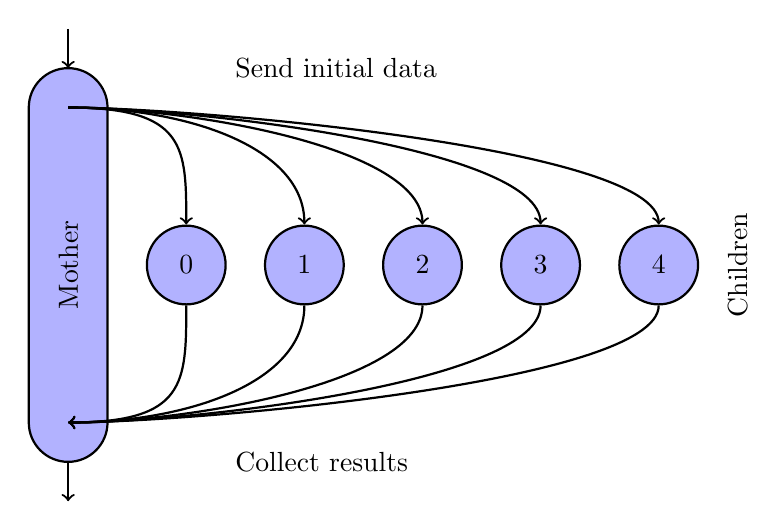
\begin{tikzpicture}
    \draw [rounded corners=0.5cm,thick,fill=intermed]
      (-0.5,2.5) rectangle (0.5,-2.5) ;
    \node [rotate=90] {Mother};

    \draw [func] (0,3) -- (0,2.5);
    \foreach \i in {0,...,4}
    {
      \node [circle,thick,fill=intermed,draw,thick,minimum height=1cm]
        (c\i) at (1.5+\i*1.5,0) {\i} ;
      \draw [func] (0,2) ..controls +(1.5,0) and +(0,1.5) .. (c\i);
      \draw [func] (c\i) ..controls +(0,-1.5) and +(1.5,0) .. (0,-2);
    }
    \node at(8.5,0) [rotate=90] {Children};
    \draw [func] (0,-2.5) -- (0,-3) ;
    \node at (2,2.5) [anchor=west] {Send initial data} ;
    \node at (2,-2.5) [anchor=west] {Collect results} ;
  \end{tikzpicture}
  \end{center}

  \bigskip
  (formerly called ``Master-Slave'')
\end{frame}
% }}}
% -----------------------------------------------------------------------------
\subsection{Partition}
% -----------------------------------------------------------------------------
% {{{
\begin{frame}{Partition}
  {\Huge
  \[
    y_i = f_i(x_{i-1}, x_i, x_{i+1})
  \]}
  where $i\in\{1,\dots,N\}$.

  \pause
  \bigskip
  Includes straightforward
  generalizations to dependencies on a larger (but
  not $O(P)$-sized!) set of neighbor inputs.

  \pause
  \bigskip
  \textbf{Point:} Processor $i$ \emph{owns} $x_i$. (``owns'' = is
  ``responsible for updating'')
\end{frame}
% -----------------------------------------------------------------------------
\begin{frame}{Partition: Graph}
  \begin{center}
    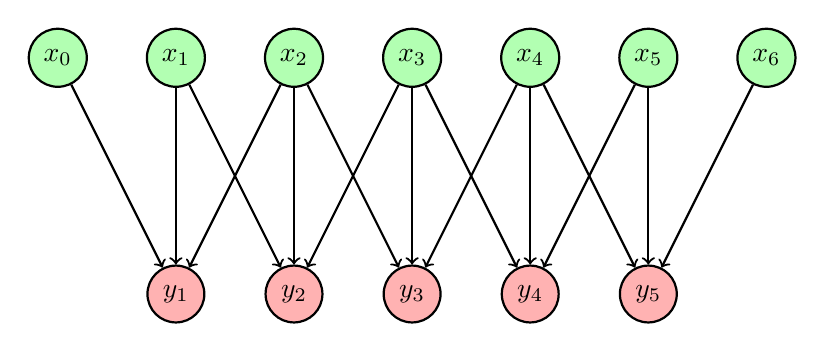
\begin{tikzpicture}
      \foreach \i in {0,...,6}
      {
        \node [input] at (1.5*\i, 0) (x\i) { $x_{\i}$ };
      }
      \foreach \i in {1,...,5}
      {
        \node [output] at (1.5*\i, -3) (y\i) { $y_{\i}$ };
      }
      \foreach \i in {1,...,5}
      {
        \pgfmathtruncatemacro{\iminusone}{\i-1}
        \pgfmathtruncatemacro{\iplusone}{\i+1}
        \draw [func] (x\i) -- (y\i) ;
        \draw [func] (x\iminusone) -- (y\i) ;
        \draw [func] (x\iplusone) -- (y\i) ;
      }
    \end{tikzpicture}
  \end{center}
\end{frame}
% -----------------------------------------------------------------------------
\begin{frame}{Mapping to Mechanisms}
  \begin{itemize}[<+->]
    \item OpenMP?
    \item MPI?
    \item MPI: Larger than \# ranks?
    \item GPU?
  \end{itemize}
\end{frame}
% -----------------------------------------------------------------------------
\begin{frame}{Partitioning for neighbor communication}
  \begin{center}
    \includegraphics[height=7cm]{mesh-partition.png}
  \end{center}
  \uncover<+>{}
  \uncover<+->{
    \begin{tikzpicture} [overlay]
      \node [above left=0.5cm of current page.south east, draw,drop shadow,fill=white,
      inner xsep=0.5cm,inner ysep=0.5cm,thick]
        {
          How can I chop up a domain?
        } ;
    \end{tikzpicture}
  }
\end{frame}

\questionframe{}
\imagecreditslide

\end{document}
% vim: foldmethod=marker

